\begin{titlepage}

    \centering
    
    \begin{tikzpicture}
    	
    	\node[inner sep=0pt] (logo) at (0,0)
    	{
\includegraphics[width=.30\textwidth]{Figures/1. STP/eilco.png}};
    	
   \end{tikzpicture}
\vspace{3cm}	
    
    \begin{tikzpicture}
    
   \node[inner sep=0pt] (logo) at (0,0)
   {
\includegraphics[width=.25\textwidth]{Figures/1. STP/eilco.png}};
   
    
    \node[inner sep=0pt] (logo) at (0,0)
        {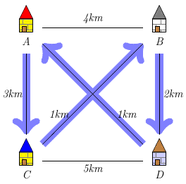
\includegraphics[width=.25\textwidth]{Figures/1. STP/stp.png}};
        
    \node[text width = 0.5\textwidth, right = of logo](title){\sffamily\huge\reporttitle};
    
    \node[text width = 0.5\textwidth, yshift = 0.75cm, below = of title](subtitle){\sffamily\Large \reportsubtitle};
    
    \gettikzxy{(subtitle.south)}{\sffamily\subtitlex}{\subtitley}
    \gettikzxy{(title.north)}{\titlex}{\titley}
    \draw[line width=1mm, Tue-red]($(logo.east)!0.5!(title.west)$) +(0,\subtitley) -- +(0,\titley);
    
    \end{tikzpicture}
    \vspace{3cm}
    
  
    
    \begin{table}[H]
    \centering
     \LARGE
    \begin{tabu} to 0.8\linewidth {cc}
    \textbf{Etudiant} :  \LARGE \reportauthors
    
    \end{tabu}
    
    \end{table}
    
     \textbf{Professeure:} \LARGE  \tutor
    
    \tikz[remember picture,overlay]\node[anchor=south,inner sep=0pt] at (current page.south) {
\includegraphics[width=\paperwidth]{Figures/0. General/pied2.jpg}};
    
    \mbox{}
    \vfill
    \iffalse
    \sffamily \Large \textcolor{white}{\placeanddate} \\
    \fi
    
    
    
    \end{titlepage}
    
    
    
    
    
    
    
    
    